\clearpage
\section{Firmware Architecture and Organization}
\label{sec:firmware_architecture}

% This section summarises the principal hardware components used in the H.E.R.A system and classifies them according to their operational roles. The objective is to provide a concise inventory of the devices, including their names, quantities, and primary functions, and then distinguish clearly between input and output hardware.



% \subsection{Introduction to OhStem's YoloUNO and AIoT Kit}

% % In this project, the central embedded controller responsible for managing the hardware subsystem is the \href{https://ohstem.vn/product/yolo-uno/}{Ohstem Yolo UNO development board}. This board serves as the local ``brain'' of the system, coordinating sensor data acquisition, communication with the upper software layer, and control of output devices such as the LCD, LED, fan, and relay. The Yolo UNO is built around a customised ESP32-S3 platform provided by \href{https://ohstem.vn/}{Ohstem}, which combines the processing capability of the ESP32-S3 with a development-friendly hardware design suitable for rapid prototyping and IoT applications.

% % The ESP32-S3 is a powerful dual-core microcontroller developed by Espressif Systems, built on the Xtensa LX7 architecture with two 32-bit CPU cores operating at up to 240~MHz. It features comprehensive wireless connectivity including Wi-Fi 802.11 b/g/n (2.4~GHz) and Bluetooth 5.0 (LE), making it ideal for IoT applications requiring robust wireless communication capabilities. \\

% % For this project, we use the ESP32-S3-N16R8 variant integrated on the Ohstem Yolo UNO development board. The N16R8 configuration provides 16~MB of flash memory and 8~MB of PSRAM, offering substantial storage and processing capabilities for complex IoT applications. The Yolo UNO board simplifies development with its built-in sensors, connectivity options and user-friendly interface, enabling seamless integration with the CoreIoT platform for data transmission and remote device control.

% In this project, the hardware subsystem is managed by the \href{https://ohstem.vn/product/yolo-uno/}{Ohstem Yolo UNO development board}, which acts as the central embedded controller of the H.E.R.A system. It is responsible for acquiring sensor data, communicating with the upper software layer, and controlling output devices such as the LCD, LED, fan, and relay. Developed by \href{https://ohstem.vn/}{Ohstem}, the Yolo UNO is based on a customised ESP32-S3 platform and is designed to support rapid prototyping and IoT-oriented applications through its integrated peripherals and development-friendly architecture. \\

% At its core, the ESP32-S3 is a high-performance dual-core microcontroller from Espressif Systems, built on the Xtensa LX7 architecture with two 32-bit processors operating at up to 240~MHz. It also provides built-in Wi-Fi 802.11 b/g/n (2.4~GHz) and Bluetooth 5.0 Low Energy connectivity, which makes it well suited for wireless embedded systems. \\

% The specific version used in this project is the ESP32-S3-N16R8, which provides 16~MB of flash memory and 8~MB of PSRAM. This memory configuration offers sufficient capacity for firmware development, wireless communication, sensor integration, and interaction with the CoreIoT platform for remote monitoring and device control.

% \begin{figure}[H]
%     \centering
%     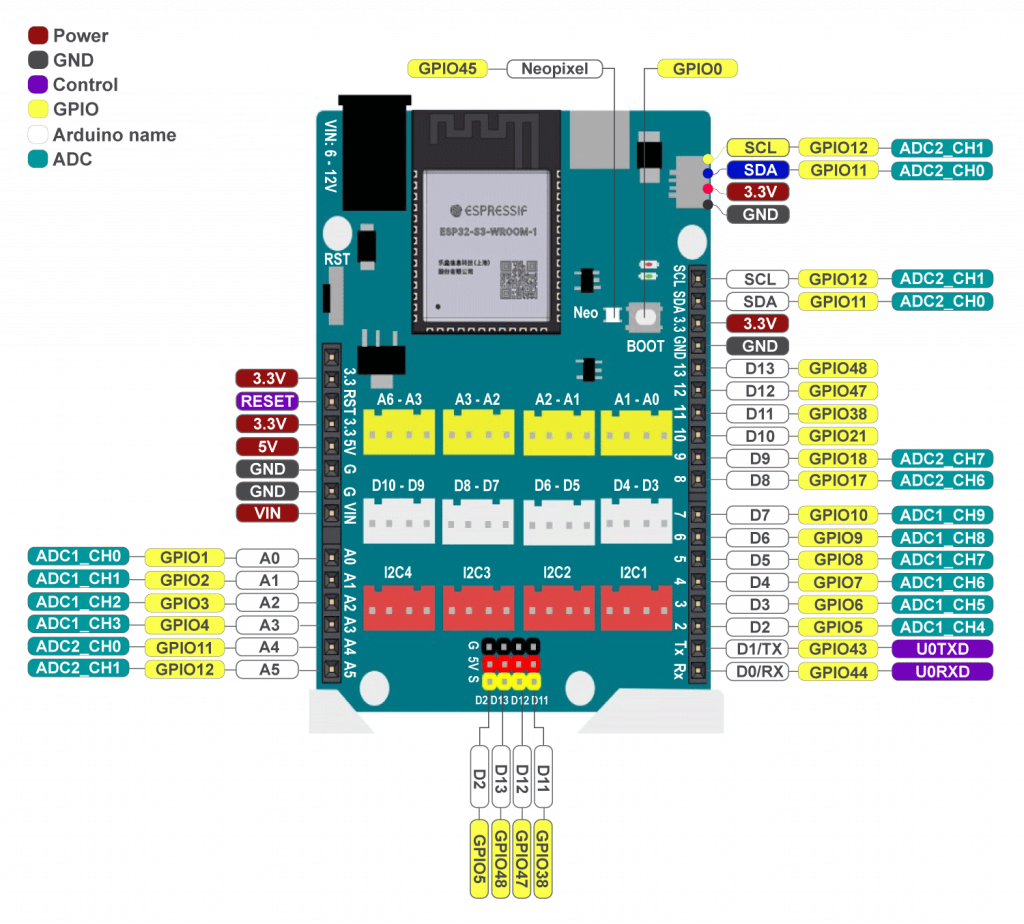
\includegraphics[width=0.95\linewidth]{image/figure/pinout-mach-yolo-uno.png}
%     \caption{ESP32-S3-N16R8 based Ohstem Yolo UNO development board and pinout.}
%     \label{fig:yolouno_esp32s3_pinout}
% \end{figure}

% In project, we will use PlatformIO to develop and upload firmware to the ESP32-S3 microcontroller on the Yolo Uno board. PlatformIO is an open-source ecosystem for IoT development that supports multiple platforms and frameworks, providing a unified interface for building, testing, and deploying embedded applications.






\subsection{Introduction to OhStem's Yolo UNO and AIoT Kit}

In this project, the hardware subsystem is centred around the \href{https://ohstem.vn/product/yolo-uno/}{Ohstem Yolo UNO development board}, which serves as the main embedded controller of the H.E.R.A system. As the local control unit, it is responsible for acquiring sensor data, communicating with the upper software layer, and executing control commands for output devices such as the LCD, RGB LED, fan, and relay. Developed by \href{https://ohstem.vn/}{Ohstem}, the Yolo UNO is built on a customised ESP32-S3 platform and is intended to support rapid prototyping, embedded control, and IoT-oriented application development through its user-friendly and integration-ready design. \\

At the core of the Yolo UNO is the ESP32-S3, a high-performance dual-core microcontroller developed by Espressif Systems. Based on the Xtensa LX7 architecture, it features two 32-bit processors operating at up to 240~MHz, together with built-in Wi-Fi 802.11 b/g/n (2.4~GHz) and Bluetooth 5.0 Low Energy connectivity. These capabilities make it well suited for intelligent embedded systems that require reliable wireless communication and real-time interaction with external devices. \\

The specific version used in this project is the ESP32-S3-N16R8, which provides 16~MB of flash memory and 8~MB of PSRAM. This hardware configuration offers sufficient resources for firmware development, peripheral integration, wireless communication, and interaction with the CoreIoT platform for remote monitoring and device control.

\begin{figure}[H]
  \centering
  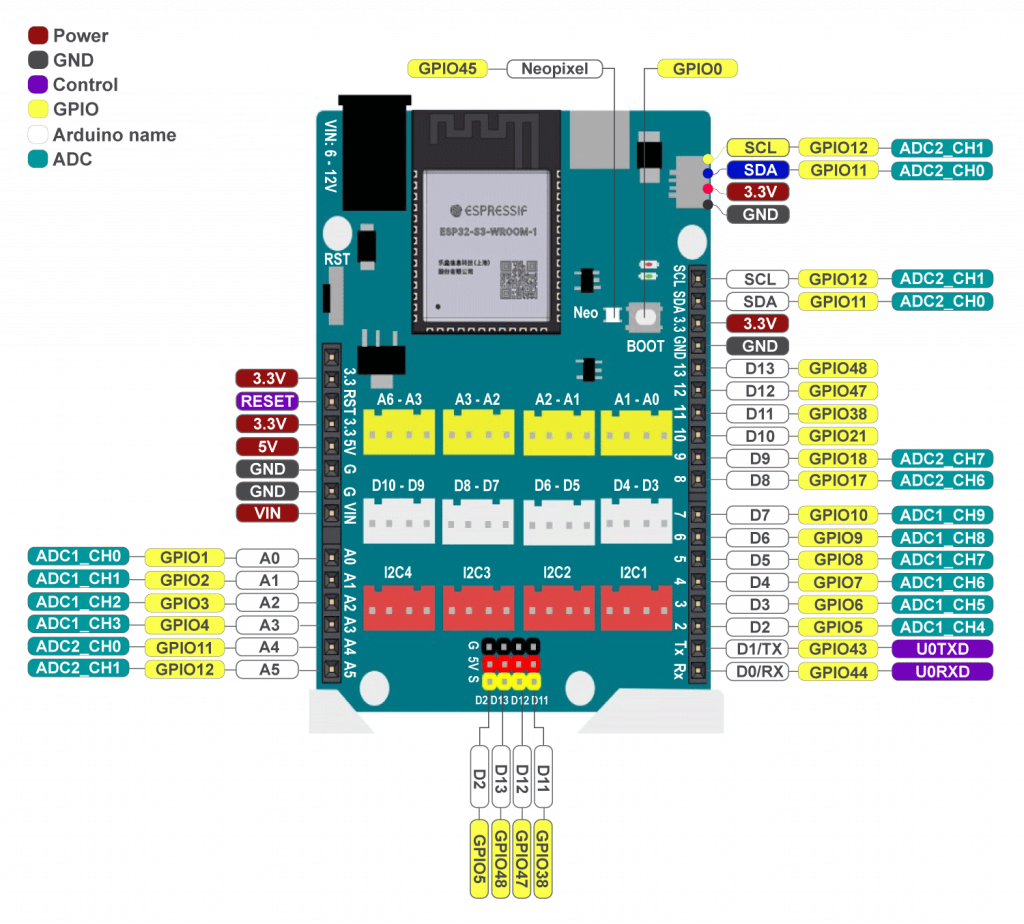
\includegraphics[width=0.95\linewidth]{image/figure/pinout-mach-yolo-uno.png}
  \caption{ESP32-S3-N16R8 based Ohstem Yolo UNO development board and pinout.}
  \label{fig:yolouno_esp32s3_pinout}
\end{figure}

For firmware development and deployment, this project uses PlatformIO to program the ESP32-S3 microcontroller on the Yolo UNO board. PlatformIO is an open-source ecosystem for IoT development that supports multiple platforms and frameworks, providing a unified environment for building, uploading, testing, and maintaining embedded applications. \\

In addition to the controller board itself, many of the peripheral devices used in the system, including input modules, output modules, and environmental sensors, are selected from the \href{https://ohstem.vn/product/aiot-kit-hoc-lap-trinh-iot-va-ai/}{OhStem AIoT Kit}. This kit provides a convenient collection of plug-and-play modules, allowing the hardware components of the H.E.R.A system to be integrated more easily, safely, and consistently during development and experimentation.

\begin{figure}[H]
  \centering
  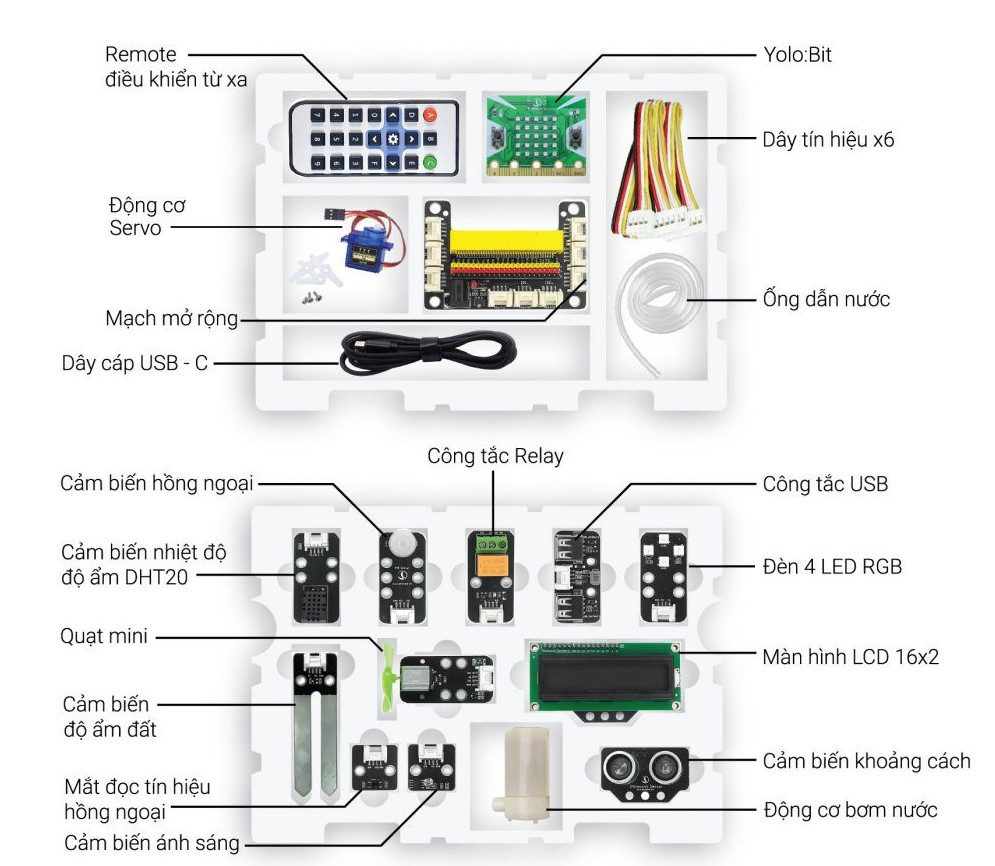
\includegraphics[width=0.95\linewidth]{image/figure/kit-hoc-lap-trinh-IoT-va-AI-AIoT-Kit.jpg}
  \caption{OhStem AIoT Kit and its main hardware modules.}
  \label{fig:ohstem_aiot_kit}
\end{figure}

Figure~\ref{fig:ohstem_aiot_kit} shows the OhStem AIoT Kit, which provides a set of plug-and-play modules for IoT and embedded-system prototyping. The kit includes a variety of common input and output devices, such as the DHT20 sensor, infrared modules, light sensor, relay, RGB LED, LCD display, mini fan, ultrasonic sensor, and water pump. \\

In the H.E.R.A system, the AIoT Kit serves as the main source of peripheral modules for sensing and actuation. Its modular design simplifies hardware integration and supports faster, safer, and more convenient prototype development.





\newpage
\subsection{Hardware Device Inventory}

\begin{table}[htbp]
  \centering
  \caption{Main hardware devices used in the H.E.R.A system}
  \label{tab:hardware_inventory}
  \renewcommand{\arraystretch}{1.2}
  \small
  \begin{tabularx}{\textwidth}{|>{\centering\arraybackslash}p{0.8cm}|p{4.0cm}|>{\centering\arraybackslash}p{1.0cm}|X|}
    \hline
    \textbf{No.} & \textbf{Device Name} & \textbf{Qty.} & \textbf{Primary Function} \\
    \hline \hline
    1  & Central Processing Node (PC) & 1 & Performs high-level processing tasks, including Speech-to-Text (STT), Natural Language Understanding (NLU), and command coordination for the overall system. \\
    \hline
    2  & Microphone / Sound Sensor & 1 & Captures user voice input for speech-based interaction and forwards audio data to the processing layer. \\
    \hline
    3  & Yolo UNO Development Board & 1 & Serves as the main embedded controller, handling sensor data acquisition, MQTT communication, and actuator control. \\
    \hline
    4  & Temperature and Humidity Sensor (DHT20) & 1 & Measures ambient temperature and humidity for environmental monitoring and automated control decisions. \\
    \hline
    5  & Light Sensor (LDR) & 1 & Detects surrounding light intensity to support context-aware lighting automation. \\
    \hline
    6  & LCD Display & 1 & Displays real-time sensor readings, device states, and general system status information. \\
    \hline
    7  & RGB LED Module (WS2812) & 1 & Provides visual output for lighting control demonstration and system status indication. \\
    \hline
    8 & Mini Fan & 1 & Simulates ventilation or cooling control in response to environmental conditions or user commands. \\
    \hline
    9 & Relay Module & 1 & Enables switching control of external electrical loads or household appliances. \\
    \hline
  \end{tabularx}
\end{table}

\subsection{Functional Classification of Hardware Devices}

To provide a clearer view of the hardware architecture, the devices used in the H.E.R.A system can be classified according to their functional roles. Rather than considering only input and output functions, this classification also includes the processing and control units that coordinate sensing, communication, and actuation within the system.

\begin{table}[H]
  \centering
  \caption{Functional classification of hardware devices in the H.E.R.A system}
  \label{tab:functional_classification}
  \renewcommand{\arraystretch}{1.2}
  \small
  \begin{tabularx}{\textwidth}{|p{2.2cm}|p{4.0cm}|X|}
    \hline
    \textbf{Category} & \textbf{Devices} & \textbf{Role in the System} \\
    \hline \hline
    Processing and Control Units
    & Central Processing Node (PC), Yolo UNO Development Board
    & These units form the computational and control core of the system. The PC performs high-level processing tasks such as speech recognition, natural language understanding, and command orchestration, while the Yolo UNO executes embedded control tasks including sensor acquisition, MQTT communication, and actuator management. \\
    \hline
    Input Devices
    & DHT20 temperature and humidity sensor, LDR light sensor
    & These devices collect environmental data, specifically temperature, humidity, and ambient light intensity, then forward it to the controller for processing and decision-making. \\
    \hline
    Output Devices
    & LCD display, RGB LED module, mini fan, relay module
    & These devices present system information and perform physical responses, such as visual feedback, airflow generation, and switching external electrical loads or appliances. \\
    \hline
  \end{tabularx}
\end{table}

In summary, the H.E.R.A platform combines sensing devices, embedded control hardware, and output actuators into an integrated smart-home architecture. This functional organisation enables the system not only to perceive environmental conditions and user input, but also to process commands intelligently and respond through appropriate physical actions.





\subsection{Software Environment}

The software environment and main libraries used in this project (which are already included) are:

\begin{itemize}
  \item PlatformIO plug-in with the right toolchain.
  \item FreeRTOS as the real-time operating system.
  \item C/C++ as the main programming language for embedded tasks.
  \item Libraries for the DHT20 sensor, NeoPixel (Adafruit NeoPixel or equivalent), and I\textsuperscript{2}C LCD.
  \item (python model ghi vô đây).
  \item (Docker ghi vô đây)
  \item Python 3.8.5 environment for data collection, cleaning, and model training.
  \item Telegram Bot API accessed from Python scripts.
\end{itemize}


\newpage
\subsection{Firmware Directory Structure}

\subsubsection{Firmware Directory Tree}

\begin{lstlisting}[style=projecttree]
MP-AI-252/                       # Root directory of the project workspace
|-- firmware/                    # Embedded firmware for the ESP32-based device
|   |-- boards/                  # Custom board definitions for PlatformIO
|   |-- data/                    # Filesystem data stored on the board
|   |-- include/                 # Header files for shared modules and drivers
|   |-- lib/                     # Local and third-party embedded libraries
|   |   |-- DHT20/               # Driver library for the DHT20 sensor
|   |   |-- LCD/                 # Driver library for the LCD display
|   |   `-- PubSubClient/        # MQTT client library for device communication
|   |-- src/                     # Main implementation source files
|   `-- test/                    # Test folder for firmware modules
|
|-- BE/                          # Backend services and AI processing modules
|   |-- Database/                # Database scripts and backend server setup
|   |-- HERA/                    # Core multi-agent AI assistant backend
|   |   |-- adapters/            # Adapters for external communication channels
|   |   |-- agents/              # AI agents for different system tasks
|   |   |-- core/                # Shared core logic and system services
|   |   `-- ...
|   |-- MQTT_Broker/             # MQTT broker, simulator, and test utilities
|   |-- Telegram Bot/            # Utilities for Telegram-based messaging
|   `-- omniverse/               # Omniverse assets and related resources
|
|-- FE/                          # Frontend applications and user interfaces
|   |-- board-host/              # Lightweight web UI for board interaction
|   `-- hera-dashboard/          # Main dashboard for monitoring and control
|       |-- public/              # Static assets served directly by the app
|       `-- src/                 # Main source code of the frontend
|           |-- assets/          # Images, icons, and static resources
|           |-- components/      # Reusable UI components
|           |-- pages/           # Page-level views of the application
|           `-- services/        # API calls and service logic
|
|-- docs/                        # Documentation and LaTeX report sources
|   |-- content/                 # LaTeX section files for report chapters
|   |-- image/                   # Figures, plots, and visual assets
|   `-- report/                  # Report project and compiled outputs
|
|-- .gitignore                   # Git ignore rules for generated and temporary files
|-- platformio.ini               # PlatformIO project configuration file
|-- README.md                    # Main overview and usage guide of the project
`-- run_full_pipeline.sh         # Shell script to run the full system pipeline
\end{lstlisting}


\subsubsection{Description of Main Directories and Files}

The project is organized into several main folders and configuration files in the root working directory:

\begin{itemize}
  \item \texttt{\textbf{platformio.ini}}: PlatformIO project configuration file, including board settings, framework options, and embedded library dependencies for firmware development.
  \item \texttt{README.md}: the main project overview, describing the purpose of the system, its modules, and usage instructions.
  \item \texttt{run\_full\_pipeline.sh}: shell script for executing the full system pipeline, typically used to automate multi-stage tasks across project modules.
  \item \texttt{tomtat.md}: summary notes or a concise project overview used for quick reference.
  \item \texttt{.gitignore}: Git configuration file specifying generated, temporary, and environment-specific files to be excluded from version control.
\end{itemize}

The main directories are:

\begin{itemize}
  \item \textbf{firmware/}: embedded firmware source tree for the ESP32-based device. This module contains the low-level logic for device control, sensor acquisition, communication, and local peripherals.
    \begin{itemize}
      \item \textbf{boards/}: custom PlatformIO board definition files, including the configuration for the \texttt{yolo\_uno} board.
      \item \textbf{data/}: board filesystem data used for deployment to the embedded device when required.
      \item \textbf{include/}: C/C++ header files for shared interfaces, hardware abstractions, and manager modules. The folder is further divided into:
        \begin{itemize}
          \item \textbf{devices/}: abstractions and controllers for actuators and output devices, such as binary-state devices, WS2812 LEDs, and actuator management.
          \item \textbf{sensors/}: abstractions and interfaces for supported sensors, including DHT20- and MQ2-related sensor modules.
          \item Shared headers such as \texttt{global.h}, \texttt{main.h}, \texttt{mqtt\_handle.h}, \texttt{analog\_manager.h}, \texttt{digital\_manager.h}, \texttt{LCD\_display.h}, \texttt{ir\_receiver.h}, \texttt{led\_display.h}, and \texttt{neo\_display.h} provide declarations for common system components.
        \end{itemize}
      \item \textbf{lib/}: local reusable libraries and third-party embedded dependencies, including:
        \begin{itemize}
          \item \textbf{DHT20/}: driver implementation for the DHT20 sensor.
          \item \textbf{LCD/}: LCD driver library for display handling.
          \item \textbf{PubSubClient/}: MQTT client library used for network-based device communication.
        \end{itemize}
      \item \textbf{src/}: main firmware implementation files, including source code for display handling, analog/digital management, global resource initialization, MQTT communication, infrared input, NeoPixel output, and sensor acquisition.
      \item \textbf{test/}: auxiliary test directory for firmware-related experiments and validation.
    \end{itemize}

  \item \textbf{BE/}: backend and AI service layer of the system. This module groups the data, communication, orchestration, and intelligent assistant components used by the overall platform.
    \begin{itemize}
      \item \textbf{Database/}: database initialization and backend server scripts, including package configuration and server-side setup files such as \texttt{init\_dbs.js} and \texttt{server.js}.
      \item \textbf{HERA/}: the core multi-agent AI assistant backend. This folder is structured into several submodules:
        \begin{itemize}
          \item \textbf{adapters/}: communication adapters for external interaction channels, such as Telegram and voice-based interfaces.
          \item \textbf{agents/}: specialized agents responsible for different tasks, including anomaly detection, chat handling, device interaction, orchestration, and sensor-related reasoning.
          \item \textbf{core/}: shared backend services and infrastructure, including the event bus, language policy, LLM service, message representation, MQTT service, and tool registry.
          \item Additional files such as \texttt{main.py}, \texttt{hera\_bot.py}, \texttt{config.py}, and \texttt{omniverse\_connector.py} define the main application entry points and runtime configuration of the HERA backend.
        \end{itemize}
      \item \textbf{MQTT\_Broker/}: lightweight MQTT infrastructure and utilities, including broker logic, publisher/subscriber examples, simulator scripts, and test programs for validating message-based communication.
      \item \textbf{Telegram Bot/}: helper scripts for Telegram-based messaging and notification features.
      \item \textbf{omniverse/}: assets and scene resources related to Omniverse integration.
    \end{itemize}

  \item \textbf{FE/}: frontend applications and user-facing interfaces. This module contains the web-based components used for local control and system monitoring.
    \begin{itemize}
      \item \textbf{board-host/}: lightweight local web interface consisting of static files such as \texttt{index.html}, \texttt{script.js}, and \texttt{styles.css}, used for direct interaction with the board.
      \item \textbf{hera-dashboard/}: the main frontend dashboard for the HERA system, developed as a modern web application.
        \begin{itemize}
          \item \textbf{public/}: static public assets such as icons and favicon resources.
          \item \textbf{src/}: main source code of the dashboard frontend, further divided into:
            \begin{itemize}
              \item \textbf{assets/}: images, icons, and other static UI resources.
              \item \textbf{components/}: reusable user interface components.
              \item \textbf{pages/}: page-level views and route targets.
              \item \textbf{services/}: service-layer code for API calls and frontend--backend communication.
            \end{itemize}
          \item Files such as \texttt{App.jsx}, \texttt{main.jsx}, \texttt{index.css}, \texttt{package.json}, \texttt{tailwind.config.js}, and \texttt{vite.config.js} define the application structure, styling system, package dependencies, and build configuration.
        \end{itemize}
    \end{itemize}

  \item \textbf{docs/}: documentation and report-writing resources for the project.
    \begin{itemize}
      \item \textbf{content/}: LaTeX section files for individual report chapters, such as introduction, requirement analysis, device description, multi-AI architecture, TinyML/personalization, and database sections.
      \item \textbf{image/}: figures, plots, diagrams, and other graphical assets used in the report.
      \item \textbf{report/}: a standalone report workspace containing content files, style files, images, build artifacts, and compiled output such as the final PDF.
      \item Additional root files such as \texttt{main.tex}, \texttt{main.pdf}, \texttt{HOW\_TO\_COMPILE.md}, and \texttt{BUILD\_AND\_RENDER.bat} support report authoring and compilation.
    \end{itemize}
\end{itemize}


\newpage
\subsection{Configuration Macros and System Modes}

An important design decision is the introduction of a centralized configuration header (included at the beginning of \texttt{global.h}) that defines all operational parameters using preprocessor macros. This header groups together:

\begin{itemize}
  \item \textbf{Mode flags}: debug and logging options (e.g., enabling or disabling debug output and payload display).
  \item \textbf{Task delays and timeouts}: delays for LED blinking, NeoPixel updates, sensor reading, TinyML inference, CoreIOT publishing, and Wi-Fi/MQTT retry intervals.
  \item \textbf{GPIO mappings}: pins for the on-board LED, NeoPixel data line and LED count.
  \item \textbf{I\textsuperscript{2}C pins}: SDA and SCL GPIO mapping for the LCD module and other I\textsuperscript{2}C peripherals.
\end{itemize}

An excerpt of the configuration header is shown below:

\begin{lstlisting}[language=C,caption={Excerpt of configuration macros}]
// ----- General Settings -----
// Mode Settings
#define IS_DEBUG_MODE               false
#define IS_MONITOR_MODE             false
#define IS_SHOW_DHT20_STATUS        false
#define IS_SHOW_LED_STATUS          false
#define IS_SHOW_DIGITAL_STATUS      false
#define IS_SHOW_ANALOG_STATUS       false
#define IS_SHOW_BUTTON_STATUS       false
#define IS_SHOW_NEO_STATUS          false
#define IS_SHOW_LCD_STATUS          false
#define IS_SHOW_PAYLOAD             false
#define IS_SHOW_INFERENCE_RESULT    false

#define IS_SHOW_MQ2_STATUS          false
#define IS_SHOW_BOT_STATUS          false
#define IS_SHOW_SENSOR_LOG          false

// Time Delays (in milliseconds)
#define LED_BLINKY_DELAY_MS         1000
#define NEO_DISPLAY_DELAY_MS        1000
#define TEMP_HUMI_DELAY_MS          1000
#define MAIN_SERVER_DELAY_MS        1000
#define TINY_ML_DELAY_MS            5000
#define POLL_FROM_SERVER_DELAY_MS   1000
#define CORE_IOT_DELAY_MS           10000

#define LED_READER_DELAY_MS         1000
#define HUMID_READER_DELAY_MS       1000

#define LONG_PRESS_MS               3000
#define DEBOUNCE_MS                 50

#define ANALOG_READ_DELAY_MS        10
#define ANALOG_DEBOUNCE_MS          80

#define WIFI_CONNECT_TIMEOUT_MS     10000
#define WIFI_RETRY_INTERVAL_MS      5000
#define MQTT_RETRY_INTERVAL_MS      5000
#define SENSOR_LOG_DELAY_MS         2000
#define GAS_MONITOR_DELAY_MS        2000
// ----- END General Settings -----

// ----- Board default ports mapping -----
// Digital Grove Ports
#define DIGITAL_PORT_1_PIN          18      // D9
#define DIGITAL_PORT_2_PIN          10      // D7
#define DIGITAL_PORT_3_PIN          8       // D5
#define DIGITAL_PORT_4_PIN          6       // D3

#define DIGITAL_PORT_1_SUB_PIN      21      // D10
#define DIGITAL_PORT_2_SUB_PIN      17      // D8
#define DIGITAL_PORT_3_SUB_PIN      9       // D6
#define DIGITAL_PORT_4_SUB_PIN      7       // D4

// Analog Grove Ports
#define ANALOG_PORT_1_PIN           4       // A3
#define ANALOG_PORT_2_PIN           3       // A2
#define ANALOG_PORT_3_PIN           2       // A1
#define ANALOG_PORT_4_PIN           1       // A0

// I2C Pins
#define I2C_SDA_PIN                 11      // A4
#define I2C_SCL_PIN                 12      // A5
// ----- END Board default ports mapping -----

// ----- GPIO Pins Definitions -----
// Buttons
#define BOOT_PIN                    0
#define BUTTON_PIN                  47

// Grove's port devices
#define WS2812_PIN                  DIGITAL_PORT_1_PIN
#define IR_RECEIVE_PIN              DIGITAL_PORT_2_PIN
#define MINI_FAN_PIN                DIGITAL_PORT_3_PIN
#define RELAY_PIN                   DIGITAL_PORT_4_PIN

#define ANALOG_GPIO_PIN             ANALOG_PORT_1_PIN
#define LIGHT_SENSOR_PIN            ANALOG_PORT_2_PIN
#define MQ2_SENSOR_PIN              ANALOG_PORT_3_PIN
#define SOIL_MOISTURE_PIN           ANALOG_PORT_4_PIN

// GPIO ports
#define LED_PIN                     48

#define NEO_LED_PIN                 45
#define NEO_LED_NUMBER              8

#define WS2812_NUMBER               4
// ----- END GPIO Pins Definitions -----

// ----- Sensor & Device Constants -----
#define V_REF                      3.3f
// ----- END Sensor & Device Constants -----
\end{lstlisting}

At system startup, this header is compiled into all relevant modules, and the macros are used instead of hard-coded literals inside the application logic. This design allows users to adjust system behavior (timing, modes and pin mapping) by editing a single header file, without modifying the core task implementations. This centralized configuration mechanism is an explicit extended feature beyond the original assignment.
